\documentclass[10pt]{article}

\usepackage[utf8]{inputenc}
\usepackage[T2A]{fontenc}
\usepackage[russian, english]{babel}

\usepackage{amssymb, amsmath, textcomp, tabularx, graphicx}

\newcolumntype{C}{>{\centering\arraybackslash}X}%

\title{Задание 6}
\author{Коновалов Андрей, 074}
\date{}

\let \eps \varepsilon

\begin{document}

\maketitle

\noindent
\begin{tabularx}{\textwidth}{|C|C|C|C|C|C|C|}
  \hline
  0 & 1 & 2 & 3 & 4 & 5 & $\sigma$ \\
  \hline
  &&&&&& \\
  \hline
\end{tabularx}

\bigskip

{\bf Задача 2}

Сделаем переобозначение терминалов и нетерминалов в грамматике для краткости записи. $G = ( \{ s, f \}, \{ i, e, o \}, P = \{ s \rightarrow is | ifes | o; f \rightarrow ifef | o; \}, s)$.

\smallskip

{\bf (i)} По алгоритму, описанному в теории, построим N-автомат со стеком $M_{left} = ( \{ q \}, \{ i, e, o \}, \{ i, e, o, s, f \}, W, q, s, \varnothing )$,

\centerline{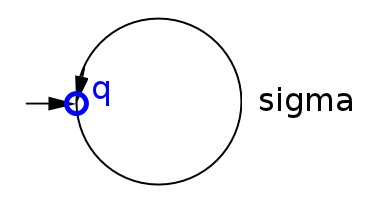
\includegraphics{image-1.png}}

\noindent $sigma = \{ (\eps, s, is), (\eps, s, ifes), (\eps, s, o), (\eps, f, ifef), (\eps, f, o), (i, i, \eps), (e, e, \eps), (o, o, \eps) \}$.

\smallskip

Допускающая последовательность конфигураций при обработке $ioeio$:

$(q, ioeio, s) \vdash (q, ioeio, ifes) \vdash (q, oeio, fes) \vdash (q, oeio, oes) \vdash (q, eio, es) \vdash (q, io, s) \vdash (q, io, io) \vdash (q, o, o) \vdash (q, \eps, \eps)$.

\smallskip

{\bf (ii)} По алгоритму, описанному в теории, построим расширенный F-автомат со стеком $M_{right} = ( \{ q, r \}, \{ i, e, o \}, \{ i, e, o, s, f, \$ \}, W, q, \$, r )$,

\centerline{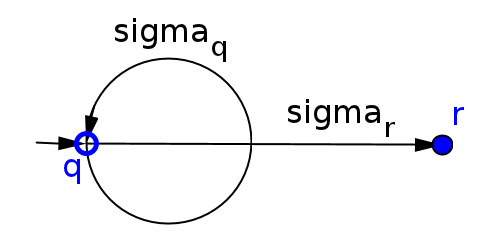
\includegraphics{image-2.png}}

\noindent $sigma_q = \{ (\eps, (is)^R, s), (\eps, (ifes)^R, s), (\eps, o, s), (\eps, (ifef)^R, f), (\eps, o, f), (i, \eps, i), \newline (e, \eps, e), (o, \eps, o) \}$, $sigma_r = \{ (\eps, s \$, \eps) \}$.

\smallskip

Допускающая последовательность конфигураций при обработке $ioeio$:

$(q, ioeio, \$) \vdash (q, oeio, i \$) \vdash (q, eio, oi \$) \vdash (q, eio, fi \$) \vdash (q, io, efi \$) \vdash (q, o, iefi \$) \vdash (q, \eps, oiefi \$) \vdash (q, \eps, siefi \$) \vdash (q, \eps, sefi \$) \vdash (q, \eps, s \$) \vdash (r, \eps, \eps)$.
\medskip

{\bf Задача 5}

{\bf (i)} Поскольку из $U$ выводимо лишь $\eps$, то из $S$ выводимы лишь слова, являющиеся перестановкой $\{ a, a, b \}$, но язык $L$ содержит и другие слова.

\smallskip

{\bf (ii)} Докажем, что КС грамматика $G$ с аксиомой $S$ и правилами вывода $\{ S \rightarrow SaSaSbS, S \rightarrow SaSbSaS, S \rightarrow SbSaSaS, S \rightarrow \eps \}$ порождает язык $L$.

\smallskip

Сначала докажем $\forall \alpha = xy \in L(G) \Rightarrow \{ x aab y, x aba y, x baa y \} \subseteq L(G)$. Пусть $\alpha \in L(G)$. Тогда существует вывод $\alpha$ в $G$. Проделаем его, пропуская все использования правила $S \rightarrow \eps$. Поскольку в правых частях остальных правил вывода между любыми двумя нетерминалами а также на концах стоит $S$, то в полученном слове между любыми двумя терминалами а также на концах будет стоять $S$. Заменим все вхождения $S$ на $\eps$, кроме одного, которое можно заменить на любое слово из $\{ SaSaSbS, SaSbSaS, SbSaSaS \}$, которое далее можно заменить на $\{ aab, aba, baa \}$ соответственно. Получаем, что $\forall x, y: xy = \alpha \Rightarrow \{ x aab y, x aba y, x baa y \} \subseteq L(G)$.

\smallskip

Теперь докажем $L(G) = L$. Включение $L(G) \subseteq L$ следует из вида правых частей правил вывода. Докажем $L \subseteq L(G)$ по индукции по количеству $n$ букв $b$ в слове $w$.

{\it База.} При $n = 0$, $\eps \in L(G)$. При $n = 1$, $\{ aab, aba, baa \} \subseteq L(G)$.

{\it Переход.} Допустим, что чисел $< n$ утверждение верно. Докажем его для $n$. Произведем в слове $w$ поиск подслов $\{ aab, aba, baa \}$. Заметим, что если вхождений не нашлось, то в любом подслове длины 3 содержится по крайней мере 2 буквы $b$, а значит $|w|_b \geq |w|_a$, чего не может быть. Получаем, что хотя бы одно вхождение хотя бы одного искомых слов $z$ нашлось. Получаем, что $w$ представимо ввиде $w = xzy$. По доказанному выше, из выводимости слова $xy$, которая выполняется по предположению индукции, следует выводимость $xzy$.

\smallskip

Теперь построим по построенной КС грамматике N-автомат со стеком $A$ по алгоритму, описанному в теории. Корректность автомата следует из корректности грамматики. $A = ( \{ q \}, \{ a, b \}, \{ a, b, S \}, W, q, S, \varnothing )$.

\centerline{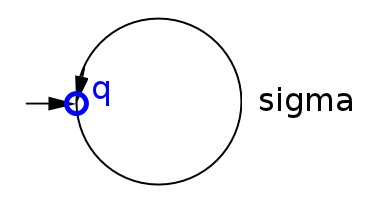
\includegraphics{image-1.png}}

\noindent $sigma = \{ (\eps, S, SaSaSbS), (\eps, S, SaSbSaS), (\eps, S, SbSaSaS), (\eps, S, \eps), (a, a, \eps), (b, b, \eps) \}$.

\smallskip

{\bf (iii)} Допускающая последовательность конфигураций $A$ при обработке слова $w = baa \in L$:

$(q, baa, S) \vdash (q, baa, SbSaSaS) \vdash (q, baa, bSaSaS) \vdash (q, aa, SaSaS) \vdash (q, aa, aSas) \vdash (q, a, SaS) \vdash (q, a, aS) \vdash (q, \eps, S) \vdash (q, \eps, \eps)$.

\smallskip

{\bf (iv)} Искомая грамматика уже была построена в пункте (ii) для построения автомата. Вывод слова $w$ в ней:

$S \rightarrow SbSaSaS \rightarrow SbSaSa \rightarrow SbSaa \rightarrow Sbaa \rightarrow baa$.

\end{document}
